\documentclass[11pt,a4paper]{article}
\usepackage[T1]{fontenc}
\usepackage{lmodern,microtype,amsmath,amssymb,mathtools,array,booktabs}
\usepackage[margin=19mm,headheight=15pt]{geometry}
\usepackage[most]{tcolorbox}
\usepackage{tikz}
\usetikzlibrary{arrows.meta,positioning,calc}
\usepackage{enumitem,fancyhdr,hyperref}
\hypersetup{colorlinks=true,linkcolor=blue!45!black,urlcolor=blue!45!black}
\setlist{itemsep=3pt,topsep=4pt,leftmargin=*}
\setlength{\parindent}{0pt}\setlength{\parskip}{5pt}
\definecolor{navy}{HTML}{14344B}\definecolor{teal}{HTML}{087E8B}
\tcbset{enhanced,breakable,boxrule=.6pt,arc=2mm,left=3mm,right=3mm,top=2mm,bottom=2mm,before skip=8pt,after skip=8pt,colback=blue!2,colframe=navy,fonttitle=\bfseries}
\newtcolorbox{concept}[1]{title={#1}}
\newtcolorbox{method}[1]{title={Method: #1},colframe=teal,colback=teal!3}
\newtcolorbox{example}[1]{title={Worked example: #1},colframe=blue!60!black,colback=blue!2}
\newtcolorbox{tip}[1]{title={Exam tip: #1},colframe=orange!80!black,colback=orange!5}
\newtcolorbox{question}[1]{title={Exam-style question #1},colframe=purple!65!black,colback=purple!3}
\newtcolorbox{answer}[1]{title={Model answer #1},colframe=green!40!black,colback=green!3}
\newcommand{\R}{\mathbb R}\newcommand{\C}{\mathbb C}\newcommand{\lap}{\mathcal L}\newcommand{\Srat}{\mathcal S}\newcommand{\dd}{\,\mathrm d}\newcommand{\ii}{\mathrm i}\newcommand{\Rea}{\operatorname{Re}}\newcommand{\I}{I}
\pagestyle{fancy}\fancyhf{}\lhead{\small MATH6321 | Mathematical Cryptography}\rhead{\small Sai Vanam}\cfoot{\thepage}
\newcommand{\F}{\mathbb F}\newcommand{\Z}{\mathbb Z}
\begin{document}
\begin{concept}{MATH6321 Mathematical Cryptography | Detailed study guide}
\Huge\textbf{Understand the idea.\\Carry out the algorithm.\\Explain the security.}\normalsize

\textbf{Prepared for Sai Vanam | 2026/27}

Based on all four supplied files: Dr Dan Fretwell's 83-page module notes, the MATH6321 exam information, Coursework 1, and the 2025 MATH320 examination with its Useful Information sheets.

This is a teaching guide and practice workbook, not an official mark scheme. Newly written questions are labelled exam-style. Actual-paper calculations and coursework examples are identified. Every topic includes explanations, a practical method, exam tips, and questions followed immediately by worked model answers.

There is a separate compact cheat sheet and editable LaTeX source. The aim is broad readiness, including unfamiliar applications; no guide can guarantee every possible future question.
\end{concept}
\begin{concept}{Read this first: the current exam guidance takes priority}
The supplied MATH6321 information specifies \textbf{two hours and five multipart questions}: Chapter 1; Chapters 2--3; Chapter 4; Chapters 5--6; Chapter 7. \textbf{No proofs are examinable.} Most work is computational, but precise descriptions, comparisons, and unseen weaknesses may be assessed. A calculator and Useful Information sheet are allowed.

The supplied 2025 MATH320 paper was \textbf{three hours, 100 marks}. It is a valuable style and calculation source, but its timing is not the current MATH6321 timing. If a future paper confirms 100 marks, a two-hour sitting gives 1.2 minutes per mark; otherwise divide the available time by the stated total.

\textbf{Learn without relying on a supplied algorithm:} Caesar, substitution, Vigenere, OTP, IoC/MutIoC, Enigma components/counting, LFSR generation/period theorems, Diffie--Hellman, RSA/signatures, Fermat, factorisation Pollard rho, BSGS, the simple noisy scheme and Gauss reduction.

\textbf{Algorithms stated to be supplied:} El-Gamal encryption/signatures, Dixon, discrete-log Pollard rho, index calculus and knapsack. You still need to execute and interpret them accurately.

\textbf{Explicitly non-examinable:} Attacking Enigma and NTRU. Short background coverage is included near the end so the whole notes structure is represented.
\end{concept}
\begin{concept}{How to use the boxes}
Blue boxes explain definitions and intuition; teal boxes give procedures; worked examples show arithmetic; orange boxes flag common errors. For practice, cover each green model answer until you have attempted its preceding question. Keep a personal error list and redo failed calculations after a gap. Proof-like justifications below explain why algorithms work; they are not a request to memorise non-examinable proofs.
\end{concept}
\tableofcontents\clearpage
\section{Essential arithmetic and notation}
\begin{concept}{The arithmetic running through the module}
\(a\equiv b\pmod n\) means \(n\mid(a-b)\). Reduce intermediate values frequently. A residue \(a\) has an inverse modulo \(n\) exactly when \(\gcd(a,n)=1\). The units form the group \((\Z/n\Z)^\times\). For a prime \(p\), its order is \(p-1\); if \(g\) generates it, powers \(g^k\) repeat with period \(p-1\).

\textbf{Keep two moduli separate:} group elements in \((\Z/p\Z)^\times\) are reduced modulo \(p\); their exponents are reduced modulo \(p-1\) (or the order of the chosen subgroup). RSA's private exponent is an inverse modulo \(\varphi(N)\), not modulo \(N\).

For letters use \(A=0,B=1,\ldots,Z=25\), except when a displayed permutation explicitly labels symbols \(1,\ldots,26\). In \(\F_2\), \(1+1=0\), so addition and subtraction both equal XOR.
\end{concept}
\begin{method}{Extended Euclid, modular equations and fast powers}
To invert \(a\pmod n\), apply Euclid to get gcd 1, then back-substitute to obtain \(ua+vn=1\). The inverse is \(u\pmod n\).

To solve \(ak\equiv b\pmod n\), let \(d=\gcd(a,n)\). If \(d\nmid b\), there is no solution. Otherwise divide the \emph{whole congruence and modulus} by \(d\), invert \(a/d\pmod{n/d}\), and recover \(d\) possible residues modulo \(n\).

To calculate \(a^e\pmod n\), write \(e\) in binary. Compute \(a,a^2,a^4,a^8,\ldots\) by repeated squaring, reducing each time, then multiply only the needed powers.
\end{method}
\begin{example}{Find the RSA inverse 11 inverse modulo 64}
\[64=5\cdot11+9,\quad11=9+2,\quad9=4\cdot2+1.\]
Back-substitute:
\[1=9-4(11-9)=5\cdot9-4\cdot11=5\cdot64-29\cdot11.\]
Thus \(11^{-1}\equiv-29\equiv35\pmod{64}\). Check: \(11\cdot35=385=6\cdot64+1\).
\end{example}
\begin{tip}{Do not divide a congruence by a nonunit}
From \(6k\equiv10\pmod{22}\), you cannot multiply by \(6^{-1}\), which does not exist. Divide by gcd 2 to get \(3k\equiv5\pmod{11}\), giving \(k\equiv9\pmod{11}\), hence \(k=9,20\pmod{22}\).
\end{tip}
\begin{question}{A.1}
Compute \(7^{-1}\pmod{26}\) and solve \(4x\equiv6\pmod{14}\).
\end{question}
\begin{answer}{A.1}
\(26=3\cdot7+5,\ 7=5+2,\ 5=2\cdot2+1\). Therefore \(1=3\cdot26-11\cdot7\), giving \(7^{-1}\equiv15\). For the second equation divide by gcd 2: \(2x\equiv3\pmod7\), so \(x\equiv4\cdot3\equiv5\pmod7\). The two residues modulo 14 are \(5,12\). Both substitute correctly.
\end{answer}
\section{Chapter 1: Caesar and monoalphabetic substitution}
\begin{concept}{Encryption, decryption and the size of the key space}
A plaintext \(m\) is encrypted as \(c=e_k(m)\), with \(d_k(e_k(m))=m\). In classical symmetric ciphers the same secret key determines encryption and decryption. Algorithms can be public; secrecy rests on the key.

\textbf{Caesar:} \(c\equiv m+k\pmod{26}\), \(m\equiv c-k\pmod{26}\). There are 26 keys, so exhaustive search is easy.

\textbf{Monoalphabetic substitution:} a permutation \(\sigma\in S_{26}\) is the key, with \(c=\sigma(m)\) and \(m=\sigma^{-1}(c)\). There are \(26!\) possible keys. This defeats a naive exhaustive search but preserves frequencies, repeated letters, word patterns and repeated words. Large key space alone does not establish security.

In cycle notation \((a\ b\ c)\) sends \(a\to b\to c\to a\). To decrypt, move \emph{backwards} in the cycle. Symbols absent from the cycles are fixed.
\end{concept}
\begin{method}{Caesar or substitution questions}
For Caesar, convert letters to numbers, add/subtract the key, reduce mod 26, and convert back. To crack it, test the 26 shifts and check a full sentence, or use a credible plaintext/ciphertext letter pair to determine \(k=c-m\).

For substitution, write an explicit ciphertext-to-plaintext table. Start with one-letter words, repeated patterns, frequent trigrams (such as THE) and likely common words. Every proposed assignment must be consistent across the whole text and injective. Verify by re-encryption; a few plausible words are insufficient evidence.
\end{method}
\begin{example}{Actual 2025 Q1(a)--(b)}
Caesar key 7 sends \(\texttt{CRYPTOGRAPHY}\) to \(\texttt{JYFWAVNYHWOF}\): for instance \(C:2\mapsto9:J\), \(Y:24\mapsto31\equiv5:F\).

The substitution key in Q1(b) uses \(1,\ldots,26\), so \(A=1\). To decrypt \(\texttt{AJQIDN}\), take predecessors in the displayed cycles:
\[A(1)\leftarrow C(3),\ J(10)\leftarrow I(9),\ Q(17)\leftarrow P(16),\]
\[I(9)\leftarrow H(8),\ D(4)\leftarrow E(5),\ N(14)\leftarrow R(18).\]
The plaintext is \(\texttt{CIPHER}\).
\end{example}
\begin{tip}{Frequency analysis is evidence, not certainty}
The most frequent letter need not represent E, especially in short texts. Combine frequency, word shapes and global consistency. The coursework explicitly rewards the explanation of cryptanalysis and awards little for plaintext alone.
\end{tip}
\begin{question}{1.1}
Encrypt \texttt{MATHS} with Caesar key 8, then decrypt \texttt{KZGXB} with key 8. Explain one weakness of substitution.
\end{question}
\begin{answer}{1.1}
\(M,A,T,H,S\) correspond to \(12,0,19,7,18\). Adding 8 gives \(20,8,1,15,0\), so \texttt{UIBPA}. Subtracting 8 from \texttt{KZGXB} gives \texttt{CRYPT}. Substitution preserves the number and pattern of occurrences of each letter: the ciphertext frequency distribution is a relabelled plaintext distribution. Enough natural-language ciphertext therefore permits statistical attacks despite \(26!\) keys.
\end{answer}
\section{Chapter 1: Vigenere, Kasiski and the one-time pad}
\begin{concept}{A repeating key versus a genuinely one-use key}
For a Vigenere key \(k=(k_1,\ldots,k_n)\), repeat the shifts periodically:
\[c_i\equiv m_i+k_{1+((i-1)\bmod n)}\pmod{26},\quad m_i\equiv c_i-k_{1+((i-1)\bmod n)}\pmod{26}.\]
A keyword is converted with \(A=0\). A plaintext letter may encrypt to several ciphertext letters, hiding a single global frequency pattern; there are \(26^n\) keys of fixed length \(n\). Repetition still creates a weakness.

Kasiski's test finds repeated ciphertext trigrams and their spacings. Repetition caused by the same plaintext under the same key alignment tends to have spacing divisible by the key length. Factor several spacings and look for a recurring divisor. Chance repetitions occur, so confirm using IoC and actual decryption.

A one-time pad has an independent uniformly random key as long as the message, kept secret and \emph{never reused}. Encryption is the same modular addition, or XOR for bits. Every candidate plaintext determines exactly one equally likely key; ciphertext alone therefore provides no extra information about the plaintext. This does not mean a nonuniform prior over plaintexts becomes uniform.
\end{concept}
\begin{method}{Execute a repeating-key encryption}
Write the plaintext, repeated keyword, numerical plaintext values, numerical key values and the resulting sum in aligned rows. Remove spaces if the cipher convention ignores them; do not accidentally advance the key for punctuation. For decryption subtract rather than add.
\end{method}
\begin{example}{Vigenere and pad reuse}
Using keyword \texttt{KEY} for \texttt{ATTACK}, the numerical rows are
\[m=(0,19,19,0,2,10),\quad k=(10,4,24,10,4,24).\]
Their sum mod 26 is \((10,23,17,10,6,8)\), giving \texttt{KXRKGI}.

For bit pads, if \(c=m\oplus k\) and \(c'=m'\oplus k\), then
\[c\oplus c'=m\oplus m'.\]
The pad cancels. Known plaintext for one message reveals \(k=c\oplus m\), and therefore decrypts the other. The analogous letter equation is \(c_i-c_i'\equiv m_i-m_i'\pmod{26}\).
\end{example}
\begin{tip}{What a comparison answer should say}
Vigenere improves on fixed substitution by varying the letter map with position and obscuring overall frequencies. It is still vulnerable to periodicity attacks. OTP eliminates that repeated-key structure when its strict randomness/one-use conditions hold, but needs a long securely distributed key. An LFSR-generated pad is deterministic and is not a true OTP.
\end{tip}
\begin{question}{1.2}
Decrypt \texttt{KXRKGI} with keyword \texttt{KEY}. Why is using the same keyword as long as the message insufficient for perfect secrecy?
\end{question}
\begin{answer}{1.2}
Subtract repeated shifts \((10,4,24,10,4,24)\) from \((10,23,17,10,6,8)\), giving \((0,19,19,0,2,10)\): \texttt{ATTACK}. Length alone does not ensure that the key is uniform, independent, secret or used only once. A human-chosen sentence-length keyword has structure and therefore fails the uniform-random requirement.
\end{answer}
\section{Chapter 1: Index of Coincidence and Mutual IoC}
\begin{concept}{Two similar statistics with different denominators}
For a string \(s\) of length \(t\ge2\), let \(N_a(s)\) count letter \(a\). Then
\[\operatorname{IoC}(s)=\frac{\sum_a N_a(s)(N_a(s)-1)}{t(t-1)}.\]
It is the probability that two \emph{distinct positions}, chosen uniformly, carry the same symbol. It is unchanged by a fixed substitution, since the counts are merely permuted. Long English-like strings typically give about \(0.0656\); independently uniform letters give expected value \(1/26\approx0.0385\).

For \emph{two} strings \(s,r\) of lengths \(t_1,t_2>0\),
\[\operatorname{MutIoC}(s,r)=\frac{\sum_aN_a(s)N_a(r)}{t_1t_2}.\]
One position is selected from each string. When \(s=r\), selection of the same position is allowed, unlike IoC. English texts encrypted with the same shift tend to yield MutIoC near \(0.0656\). Different shifts often give smaller values, but this is statistical guidance, not a deterministic test.
\end{concept}
\begin{example}{Compute both statistics carefully}
For \(s=\texttt{ABABA}\), counts are \(A:3,B:2\). Thus
\[\operatorname{IoC}(s)=\frac{3\cdot2+2\cdot1}{5\cdot4}=\frac25.\]
For \(r=\texttt{AABC}\), counts are \(A:2,B:1,C:1\), giving
\[\operatorname{MutIoC}(s,r)=\frac{3\cdot2+2\cdot1}{5\cdot4}=\frac25.\]
The equality is coincidental. For comparison \(\operatorname{MutIoC}(s,s)=(9+4)/25=13/25\), which differs from \(\operatorname{IoC}(s)\).
\end{example}
\begin{method}{Recover a Vigenere key from a MutIoC table}
For key length \(n\), split the ciphertext into columns \(s_i=c_ic_{i+n}c_{i+2n}\cdots\). Column \(i\) has shift \(k_i\). If the table shifts \(s_j\) \emph{forward} by \(\beta\), its effective key becomes \(k_j+\beta\). Alignment with \(s_i\) means
\[\boxed{\beta_{ij}\equiv k_i-k_j\pmod{26}.}\]
Pick plausible high/English-like MutIoC entries, turn them into congruences, put \(k_1=t\), and express the remaining keys in terms of \(t\). Check the unused rows for consistency, then try the 26 values of \(t\) using keyword plausibility \emph{and} decryption. Relative shifts alone leave a common Caesar shift undetermined.

For unknown key length, compare average column IoC across candidate lengths. Multiples of the true length may also look good: prefer the smallest consistent length with coherent decryption, supported by Kasiski evidence.
\end{method}
\begin{example}{Actual 2025 Q1(d): read the sign correctly}
The prominent entries occur at
\[\beta_{12}=7,\ \beta_{13}=4,\ \beta_{14}=18,\ \beta_{23}=23,\ \beta_{24}=11,\ \beta_{34}=14.\]
Set \(k_1=t\). The first three give \((k_1,k_2,k_3,k_4)=(t,t-7,t-4,t-18)\pmod{26}\). They predict \(k_2-k_3=-3\equiv23\), \(k_2-k_4=11\), \(k_3-k_4=14\), matching every remaining row. Trying the common shift \(t=4\) gives \((4,23,0,12)\), or \texttt{EXAM}, a plausible English keyword. The unused rows therefore corroborate the relative shifts, and the keyword assumption resolves the remaining common shift.
\end{example}
\begin{tip}{A high entry is not automatically an absolute key letter}
A table of MutIoC between two ciphertext columns supplies \emph{differences} between key letters. Do not read \(\beta\) directly as a keyword letter. Also do not confuse ``shift \(s_j\) forwards'' with decrypting it backwards.
\end{tip}
\begin{question}{1.3}
For \(s=\texttt{AABBC}\), calculate IoC. A length-three Vigenere key has \(\beta_{12}=25,\beta_{13}=14\), and \(k_1=10\). Find the keyword.
\end{question}
\begin{answer}{1.3}
The numerator is \(2\cdot1+2\cdot1+1\cdot0=4\), so IoC is \(4/20=1/5\). The congruences give \(k_2=10-25\equiv11\), \(k_3=10-14\equiv22\). Thus the key is \((10,11,22)\), or \texttt{KLW}. A key need not be an English word unless the question specifically assumes a keyword. Check \(10-11\equiv25\), \(10-22\equiv14\).
\end{answer}
\section{Chapter 2: Enigma components and counting}
\begin{concept}{A changing substitution with a reversible path}
A keypress sends a signal through the plugboard, the rotors, the reflector, then back through the inverse rotor path and the plugboard. The plugboard swaps disjoint pairs. Rotors permute letters; stepping changes the effective permutation from one position to another. The reflector pairs all letters and sends the signal backwards. With identical initial settings, the machine decrypts by the same process.

For a fixed rotor state, if the forward permutation is \(R\), reflector \(U\), and plugboard \(P=P^{-1}\), the overall permutation is \(P R^{-1}URP\) (rightmost map acts first). Since \(U^2=I\), the overall map is an involution. If \(U\) has no fixed points, no letter encrypts to itself. These structural restrictions helped attacks, despite the huge key space.

The module uses a simplified stepping/counting model. Answer using the assumptions stated in the question rather than adding historical ring/notch choices not requested.
\end{concept}
\begin{method}{Count independent choices without overcounting}
For \(L\) letters and exactly \(m\) disjoint plugboard pairs,
\[\boxed{\frac{L!}{(L-2m)!\,2^m m!}=\binom L{2m}(2m-1)(2m-3)\cdots1.}\]
Choose the paired letters, then pair them: divide by 2 for the order within each pair and by \(m!\) for the order of the pairs. If the number of pairs is optional, sum over permitted \(m\), including \(m=0\) if allowed.

Choose \(r\) ordered distinct rotors from \(R\): \(R!/(R-r)!\). If each has \(L\) starting positions, multiply by \(L^r\). A fully variable paired reflector on even \(L\) has \(L!/(2^{L/2}(L/2)!)\) wirings; a choice of \(h\) fixed reflectors contributes only \(h\). Multiply independent factors.
\end{method}
\begin{example}{The notes' restricted machine}
Exactly ten plug pairs on 26 letters give \(26!/(6!2^{10}10!)=150738274937250\). Three ordered rotors from five and 26 positions each give \(5\cdot4\cdot3\cdot26^3=1054560\). Choosing one of two fixed reflectors gives total
\[150738274937250\cdot1054560\cdot2=317925110435652720000.\]
Counting arbitrary rotor wirings as \((26!)^3\) is a different model and must not be mixed into this restricted count.
\end{example}
\begin{tip}{Use permutations, not combinations, for rotor slots}
Left, middle and right are distinct positions. Choosing three rotors with \(\binom53\) misses their \(3!\) orderings; equivalently use \(5\cdot4\cdot3\) directly.
\end{tip}
\begin{question}{2.1}
A toy machine has six letters, one plug pair, two ordered rotors from four, six starting positions per rotor, and one of two fixed reflectors. Count its settings.
\end{question}
\begin{answer}{2.1}
There are \(\binom62=15\) plug pairs, \(4\cdot3=12\) rotor orders, \(6^2=36\) starting positions and 2 reflectors. Their product is \(15\cdot12\cdot36\cdot2=12960\). No factorial for arbitrary rotor wiring is needed because the four available rotors are fixed.
\end{answer}
\section{Chapter 3: LFSR generation, XOR and pictures}
\begin{concept}{A small secret state produces a long deterministic stream}
An LFSR of length \(n\) has initial fill \((a_0,\ldots,a_{n-1})\in\F_2^n\) and taps \((b_0,\ldots,b_{n-1})\), with update
\[a_{i+n}=b_0a_i\oplus b_1a_{i+1}\oplus\cdots\oplus b_{n-1}a_{i+n-1}.\]
The state at time \(i\) is \((a_i,\ldots,a_{i+n-1})\); shift left and append the new bit. The output convention used here and in the notes is the stream \(a_0a_1a_2\cdots\), \emph{including the initial fill}. Encrypt bits by \(c_i=m_i\oplus a_i\); decrypt by the identical XOR.

Pictures are flattened in the specified order (the paper uses left to right, top to bottom, 0 white/1 black), XORed, then reshaped. A long period does not make a bare LFSR cryptographically secure: its linear structure can reveal states from enough known output.
\end{concept}
\begin{method}{A safe LFSR calculation table}
Write the initial bits with indices. Compute one new bit per column using the original absolute indices, never by guessing a visual pattern. For \(a_{i+5}=a_i\oplus a_{i+2}\), calculate \(a_5=a_0\oplus a_2\), then \(a_6=a_1\oplus a_3\), and so on. Keep a row of indices, stream, ciphertext and plaintext. Count the required output length before stopping.
\end{method}
\begin{example}{The 2025 paper's length-five stream}
With fill \(11010\) and \(a_{i+5}=a_i\oplus a_{i+2}\):
\[a_5=1\oplus0=1,\ a_6=1\oplus1=0,\ a_7=0\oplus0=0,\ a_8=1\oplus1=0,\ a_9=0\oplus0=0.\]
Continuing gives the first 20 bits
\[\texttt{11010 10000 10010 11001}.\]
For a ciphertext row \(\texttt{11011}\), XOR with the first five bits gives \(\texttt{00001}\). Continue with the \emph{next} five stream bits for the next row; do not restart the fill at every picture row.
\end{example}
\begin{tip}{The zero fill always stays zero}
Every feedback sum is zero, so its period is one and it provides no masking at all. Do not apply a theorem for nonzero fills to the zero fill.
\end{tip}
\begin{question}{3.1}
Use \(a_{i+3}=a_i\oplus a_{i+1}\), fill \(100\), to generate nine bits. Decrypt ciphertext \texttt{010011101}.
\end{question}
\begin{answer}{3.1}
The new bits are \(a_3=1,a_4=0,a_5=1,a_6=1,a_7=1,a_8=0\), giving stream \texttt{100101110}. XOR gives
\[\texttt{010011101}\oplus\texttt{100101110}=\texttt{110110011}.\]
Applying the same stream to this result recovers the ciphertext, since \(a_i\oplus a_i=0\).
\end{answer}
\section{Chapter 3: LFSR periods and irreducibility}
\begin{concept}{The theorems and their hypotheses}
The characteristic polynomial is
\[c_b(x)=x^n+b_{n-1}x^{n-1}+\cdots+b_1x+b_0\in\F_2[x].\]
With the notes' row-state convention, the companion matrix has ones below the diagonal and taps in its final column, and \(\mathbf a_{i+1}=\mathbf a_iB_b\).

If \(b_0=1\), \(B_b\) is invertible: the period is the first return to the initial state and divides \(\operatorname{ord}(B_b)\). Every length-\(n\) LFSR is eventually periodic; the eventual cycle has length at most \(2^n-1\). If \(b_0=0\), a transient can occur; leading untapped bits can be discarded to analyse the smaller recurrence.

\textbf{Main theorem:} if \(c_b\) is irreducible (and has nonzero constant term), every nonzero fill has the same period, the smallest positive divisor \(j\mid2^n-1\) for which \(c_b\mid x^j+1\). An irreducible polynomial is \emph{primitive} when this order is \(2^n-1\). Irreducible does not automatically mean maximal period.
\end{concept}
\begin{method}{Period questions without generating a huge stream}
\begin{enumerate}
\item Write \(c_b\) from the update rule and check its constant term.
\item Establish irreducibility if the theorem requires it. For degree 3, excluding roots 0 and 1 is enough. For degree 4, also exclude division by the only irreducible quadratic \(x^2+x+1\).
\item List divisors of \(2^n-1\) in increasing order.
\item Reduce \(x^j\) modulo \(c_b\); test for remainder 1. The first successful \(j\) is the nonzero-fill period.
\item Treat the zero fill separately. If reducible, use state iteration or another valid matrix-order argument, not the irreducible theorem.
\end{enumerate}
\end{method}
\begin{example}{Actual 2025 Q2(c)}
The recurrence \(a_{i+4}=a_i+a_{i+1}\) gives \(f=x^4+x+1\). Neither 0 nor 1 is a root. A reducible quartic with no linear factor must be a product of irreducible quadratics; the only possibility over \(\F_2\) is \((x^2+x+1)^2=x^4+x^2+1\), which differs from \(f\). Hence \(f\) is irreducible.

The possible periods divide \(15\): \(1,3,5,15\). Degree rules out dividing \(x+1\) or \(x^3+1\). The supplied factorisation
\[x^5+1=(x+1)(x^4+x^3+x^2+x+1)\]
shows that \(f\nmid x^5+1\). Thus every nonzero fill has period 15; the zero fill has period 1.
\end{example}
\begin{tip}{No roots is insufficient for a quartic}
\(x^4+x^2+1=(x^2+x+1)^2\) has no roots in \(\F_2\) but is reducible. For an irreducible quartic, periods can be 5 or 15; quote the theorem and exclude the smaller divisors.
\end{tip}
\begin{question}{3.2}
Find the period of nonzero fills when \(c_b=x^3+x+1\), and compare with \(c_b=x^4+x^3+x^2+x+1\).
\end{question}
\begin{answer}{3.2}
The cubic has no roots at 0 or 1, so is irreducible. Since \(2^3-1=7\) is prime and degree excludes order 1, every nonzero fill has period 7. For the quartic, no roots occur; it differs from \((x^2+x+1)^2\), so it is irreducible. It divides \(x^5+1\), and smaller divisors of 15 are ruled out by degree. Its nonzero-fill period is 5, not 15. Both zero fills have period 1.
\end{answer}
\section{Chapter 4: Diffie--Hellman key exchange}
\begin{concept}{Agreeing a secret without sending it}
Choose a public finite cyclic group \(G=\langle g\rangle\) of order \(q\). In the notes, a standard choice is \(G=(\Z/p\Z)^\times\), \(q=p-1\). Alice privately chooses \(a\), Bob privately chooses \(b\). They exchange \(A=g^a\), \(B=g^b\) and compute
\[K=B^a=A^b=g^{ab}.\]
An observer sees \(G,g,A,B\). Computing a discrete log would recover \(a\) or \(b\), hence the shared key. The discrete log problem asks for \(k\) with \(g^k=h\); logs are determined modulo \(q\). DH itself establishes a shared value rather than encrypting a message.

DH requires a suitable group and parameter choices. A small-order base provides only a small number of possible secrets. Basic unauthenticated DH is also vulnerable to an active intermediary who performs separate exchanges with the two parties; computational hardness alone does not authenticate identities.
\end{concept}
\begin{method}{A DH computation or explanation}
State the public group/base and private exponents, calculate both public powers by repeated squaring, then compute the shared value in both directions. Show that both equal \(g^{ab}\). For an insecure-key question, inspect the order of \(g\), trivial exponents, and whether the chosen group makes logs easy.
\end{method}
\begin{example}{A complete small exchange}
Take \(p=23,g=5,a=6,b=15\). Since \(5^2\equiv2\), \(5^4\equiv4\), Alice publishes \(A=5^6\equiv8\). Bob computes \(5^8\equiv16\), so \(B=5^{15}\equiv16\cdot4\cdot2\cdot5\equiv19\pmod{23}\).

Alice computes \(19^2\equiv16\), \(19^4\equiv3\), hence \(19^6\equiv3\cdot16\equiv2\). Bob similarly computes \(8^{15}\equiv2\). Their shared value is 2. All element arithmetic is modulo 23; exponent equivalences are modulo 22.
\end{example}
\begin{tip}{Do not claim every group makes discrete logs hard}
In the additive group \(\Z/p\Z\), the analogue of \(g^k\) is \(kg\); solving for \(k\) is just multiplying by \(g^{-1}\pmod p\). A large group size alone is insufficient.
\end{tip}
\begin{question}{4.1}
In \((\Z/11\Z)^\times\), use \(g=2,a=3,b=4\) for DH. What happens if instead \(g=-1\)?
\end{question}
\begin{answer}{4.1}
\(A=2^3=8\), \(B=2^4\equiv5\). Alice gets \(5^3=125\equiv4\); Bob gets \(8^2\equiv9\), \(8^4\equiv4\). With \(g=-1\), every public value and shared value lies in \(\{1,-1\}\). There are at most two candidate keys, so secrecy fails regardless of how large the nominal exponent range is.
\end{answer}
\section{Chapter 4: RSA encryption and insecure parameter choices}
\begin{concept}{The trapdoor is knowing the prime factors}
Choose distinct secret primes \(p,q\), set \(N=pq\) and \(\varphi(N)=(p-1)(q-1)\). Choose \(e\) coprime to \(\varphi(N)\), then calculate \(d\equiv e^{-1}\pmod{\varphi(N)}\). Public key: \((N,e)\). Private exponent: \(d\); the factors must also remain secret.

For the course's message space \(m\in(\Z/N\Z)^\times\), encrypt \(c\equiv m^e\pmod N\), decrypt \(m\equiv c^d\pmod N\). Since \(ed=1+t\varphi(N)\), Fermat--Euler gives \(m^{ed}=m(m^{\varphi(N)})^t\equiv m\). This explains correctness without being an examinable proof requirement.

Factoring \(N\) reveals \(\varphi(N)\) and \(d\). Factoring is the course's underlying hard problem; it is not a proved equivalence between every RSA attack and factorisation. These are textbook examples; deterministic unpadded RSA has additional weaknesses.
\end{concept}
\begin{method}{RSA question checklist}
\begin{enumerate}
\item Compute \(N\) and \(\varphi(N)\).
\item Check \(\gcd(e,\varphi(N))=1\). If not, no private exponent exists by the stated construction.
\item Use extended Euclid to find \(d\); verify \(ed\equiv1\).
\item Encrypt modulo \(N\) using repeated squaring.
\item Demonstrate decryption by an explicit power calculation, not only by quoting correctness.
\end{enumerate}
\end{method}
\begin{example}{Actual 2025 Q3(b): p=5, q=17, e=11}
\(N=85\), \(\varphi(N)=4\cdot16=64\), \(d=35\). Public key \((85,11)\), private exponent 35. For \(m=4\),
\[4^2=16,\quad4^4\equiv1,\quad4^8\equiv1\pmod{85},\]
so \(c=4^{11}=4^8\cdot4^2\cdot4\equiv64\pmod{85}\).

To decrypt, \(64^2=4096\equiv16\), \(64^4\equiv1\), hence \(64^{32}\equiv1\). Thus
\[64^{35}\equiv64^{32}\cdot64^2\cdot64\equiv1\cdot16\cdot64=1024\equiv4\pmod{85}.\]
\end{example}
\begin{concept}{How to spot bad RSA choices}
If two public moduli share a prime, \(\gcd(N_1,N_2)\) reveals it immediately. If primes are too close, Fermat factorisation can succeed quickly. If \(e=1\), ciphertext equals plaintext. If a positive integer message satisfies \(m^e<N\), textbook encryption does not wrap modulo \(N\), so an ordinary integer \(e\)-th root reveals \(m\). Messages \(0,1\) are obvious fixed points, and \(\gcd(m,N)>1\) itself reveals a factor (these are outside the course's unit-message assumption).
\end{concept}
\begin{tip}{Use the public data available to the attacker}
An unseen weakness answer should give a concrete procedure: ``Compute gcd of the two published moduli, divide to find each other factor, compute the totient, invert the public exponent.'' Saying merely ``the primes repeat'' leaves the attack unexplained.
\end{tip}
\begin{question}{4.2}
Two users publish \(N_1=77,N_2=91\). Explain the attack. Separately, show why \(e=6\) is invalid for primes 5 and 11.
\end{question}
\begin{answer}{4.2}
\(\gcd(77,91)=7\), so \(77=7\cdot11\), \(91=7\cdot13\). Their totients are 60 and 72. Each private exponent can now be calculated from its public exponent by modular inversion. For \(p=5,q=11\), \(\varphi(55)=40\), and \(\gcd(6,40)=2\ne1\). Thus 6 has no inverse modulo 40 and is not a valid RSA public exponent under the stated scheme.
\end{answer}
\section{Chapter 4: RSA and El-Gamal signatures}
\begin{concept}{A signature is checked with the signer's public key}
For the course's RSA auxiliary value \(m_0\), Alice signs \(\sigma\equiv m_0^d\pmod N\). Anyone with her public key verifies \(\sigma^e\equiv m_0\pmod N\). Signing uses the signer's \emph{private} exponent; encryption to a recipient uses that recipient's \emph{public} exponent.

These lecture examples are simplified textbook signatures on an auxiliary value. A signature used to authenticate document contents must be bound to those contents; the toy auxiliary-value construction alone does not provide that binding. Within exam calculations, use the supplied protocol and its notation.

For the course's El-Gamal signature in \((\Z/p\Z)^\times\), let \(q=p-1\), private key \(k\), public \(h=g^k\). Choose a fresh nonce \(s\) with \(\gcd(s,q)=1\). Then
\[m_1=g^s\pmod p,\quad m_2\equiv(m_0-km_1)s^{-1}\pmod q.\]
Verify \(h^{m_1}m_1^{m_2}\equiv g^{m_0}\pmod p\). The inverse is modulo \(q\), while the verification powers are modulo \(p\).
\end{concept}
\begin{example}{Actual 2025 Q3(c): RSA signature}
For \((N,e)=(33,3)\), \(d=7\), \(m_0=14\), compute
\[14^2\equiv31\equiv-2,\quad14^4\equiv4,\quad14^7\equiv4\cdot31\cdot14\equiv20\pmod{33}.\]
Alice sends \((14,20)\). Bob verifies \(20^2\equiv4\), so \(20^3\equiv80\equiv14\pmod{33}\), matching \(m_0\).
\end{example}
\begin{method}{El-Gamal signing in two moduli}
Make two columns on paper: ``mod \(p\): elements'' and ``mod \(p-1\): exponents''. Compute \(m_1\) first. Use its integer representative in \(m_0-km_1\), invert \(s\) modulo \(p-1\), and compute \(m_2\). Finally check both sides of the verification equation modulo \(p\).
\end{method}
\begin{tip}{Fresh nonces are essential}
For two El-Gamal signatures with the same nonce (hence the same \(m_1\)), subtraction gives \(m_2-m_2'\equiv(m_0-m_0')s^{-1}\pmod q\). This can expose \(s\) and then the private key through linear congruences. If coefficients are nonunits there may be several candidates; solve and test them rather than assuming an inverse exists.
\end{tip}
\begin{question}{4.3}
Use \(p=23,g=5,k=6\), nonce \(s=7\), and \(m_0=9\) to sign and verify an El-Gamal auxiliary value.
\end{question}
\begin{answer}{4.3}
\(h=5^6\equiv8\). The nonce is invertible modulo 22, with \(7^{-1}\equiv19\). Compute \(m_1=5^7\equiv17\), then
\[m_2\equiv(9-6\cdot17)19=-1767\equiv15\pmod{22}.\]
The signature is \((9,17,15)\). Verification: \(8^{17}\equiv13\), \(17^{15}\equiv15\pmod{23}\), so their product is \(195\equiv11\). Also \(5^9\equiv11\), hence the signature verifies.
\end{answer}
\section{Chapter 4: El-Gamal encryption}
\begin{concept}{A fresh shared mask for each message}
Choose cyclic \(G=\langle g\rangle\) of order \(q\), private \(k\), and public \(h=g^k\). The public key is \((G,q,g,h)\). To send \(m\in G\), choose fresh secret \(s\) and send
\[c_1=g^s,\qquad c_2=mh^s.\]
The recipient computes \(m=c_2c_1^{-k}\), because \(c_1^k=g^{sk}=h^s\). Unlike RSA's textbook deterministic map, fresh \(s\) can give different ciphertexts for the same message. If \(s\) is reused, \(c_2(c_2')^{-1}=m(m')^{-1}\): the common mask cancels.

A discrete log of public \(h\) recovers \(k\), hence breaks the scheme. The underlying group must make the relevant exponent problems difficult; cyclicity alone is not enough.
\end{concept}
\begin{method}{El-Gamal decryption}
Compute \(c_1^k\), find its inverse in the group, and multiply it by \(c_2\). In \((\Z/p\Z)^\times\), the group operations are multiplication and modular inversion. Do not subtract the mask: that would be an additive-group protocol.
\end{method}
\begin{example}{A small message}
Let \(p=23,g=5,k=6\), so \(h=8\). For message \(m=10\) and nonce \(s=3\),
\[c_1=5^3\equiv10,\quad h^3=8^3\equiv6,\quad c_2=10\cdot6\equiv14.\]
The recipient computes \(c_1^6=10^6\equiv6\). Since \(6^{-1}\equiv4\pmod{23}\), the message is \(14\cdot4\equiv10\).
\end{example}
\begin{tip}{Encryption nonce versus signature nonce}
The encryption calculation needs a fresh secret exponent but does not require its inverse modulo \(q\). The signature formula does, so its nonce must be coprime to \(q\). Follow the correct scheme's hypotheses.
\end{tip}
\begin{question}{4.4}
In \((\Z/11\Z)^\times\), take \(g=2,k=3,m=7,s=4\). Encrypt and decrypt.
\end{question}
\begin{answer}{4.4}
\(h=2^3=8\), \(c_1=2^4\equiv5\), \(h^4\equiv4\), so \(c_2=7\cdot4\equiv6\). The recipient gets \(c_1^k=5^3\equiv4\), inverse \(4^{-1}\equiv3\), hence \(m=6\cdot3\equiv7\pmod{11}\).
\end{answer}
\section{Chapter 5: Trial division and Fermat factorisation}
\begin{concept}{Difference of squares turns a search into factors}
Trial division tests primes up to \(\sqrt N\); every composite has such a prime factor. It is easy but costly for large generic inputs.

For odd semiprime \(N=pq\), write \(N=A^2-B^2=(A-B)(A+B)\). The useful pair is \(A=(p+q)/2\), \(B=|p-q|/2\). Close factors give small \(B\), explaining Fermat's advantage on such inputs.

The notes search \(B=1,2,\ldots\) for square \(N+B^2\). An equivalent common implementation searches \(A=\lceil\sqrt N\rceil,\ldots\) for square \(A^2-N\). If a question prescribes a version, follow it. A nontrivial \emph{congruence} of squares also suffices:
\[A^2\equiv B^2\pmod N\quad\Longrightarrow\quad \gcd(A-B,N),\ \gcd(A+B,N).\]
The gcd must be strictly between 1 and \(N\). A congruence with \(A\equiv\pm B\pmod N\) gives trivial results.
\end{concept}
\begin{method}{Fermat calculation}
For an odd input, calculate \(N+B^2\) for consecutive small \(B\), or use the specified \(A\)-search. Record square/non-square results. Once a square is found, compute both factors and multiply them back to check. Deal with an even input immediately by extracting 2; check a perfect square separately.
\end{method}
\begin{example}{N=5959}
Start with \(A=\lceil\sqrt{5959}\rceil=78\). Then \(78^2-5959=125\), not a square. At \(A=79\), \(79^2-5959=282\); at \(80\), it is 441, equal to \(21^2\). Thus
\[5959=(80-21)(80+21)=59\cdot101.\]
The notes' alternative would find the same pair when \(B=21\).
\end{example}
\begin{tip}{A square congruence is not the same as an integer square root}
For factorisation by congruences, you have a pair \(A,B\) with matching squares modulo \(N\). Taking the integer square root of a reduced residue without a valid relation is not the algorithm.
\end{tip}
\begin{question}{5.1}
Factor 221 by the notes' Fermat method. Why would close RSA primes be problematic?
\end{question}
\begin{answer}{5.1}
\(221+1^2=222\), not square; \(221+2^2=225=15^2\). Hence \(221=(15-2)(15+2)=13\cdot17\). In general the successful \(B\) is half the prime gap, so a very small gap makes the notes' search short, revealing the supposedly secret RSA factors.
\end{answer}
\section{Chapter 5: Pollard rho for factorisation}
\begin{concept}{Find a collision modulo an unknown factor}
Iterate a polynomial such as \(f(x)=x^2+1\pmod N\). The residues modulo a hidden factor may collide before the residues modulo \(N\) do. A gcd of a difference can detect this without knowing the factor.

The notes permit checking \(\gcd(x_i\pm x_j,N)\). A faster low-memory implementation (Floyd's cycle approach) runs one sequence at one step per row and another at two steps:
\[x\leftarrow f(x),\qquad y\leftarrow f(f(y)).\]
Compute \(d=\gcd(|x-y|,N)\) (and optionally the plus variant used in the notes). If \(1<d<N\), factorisation succeeds. If \(d=1\), continue. If \(d=N\), it is a trivial collision: restart with another seed/polynomial or backtrack, rather than declaring \(N\) a factorisation.
\end{concept}
\begin{method}{Show a readable rho table}
Columns should be iteration, \(x\), intermediate \(f(y)\), new \(y=f(f(y))\), difference, gcd. Reduce modulo \(N\) after \emph{each} squaring. State your seed and polynomial. Stop at a nontrivial gcd and divide \(N\) by it.
\end{method}
\begin{example}{The lecture example N=143}
Start \(x_0=y_0=2\), \(f(x)=x^2+1\pmod{143}\).
\begin{center}\begin{tabular}{rrrrr}\toprule Row&\(x\)&\(y\)&\(|x-y|\)&gcd\\\midrule
1&5&26&21&1\\2&26&15&11&11\\\bottomrule\end{tabular}\end{center}
For row 2, the fast sequence goes \(26\to105\to15\), while the slow one goes \(5\to26\). Thus \(143=11\cdot13\). The second row's \(y\) requires two applications, not one.
\end{example}
\begin{tip}{There are two different Pollard rho algorithms in this module}
Factorisation rho ends with a gcd yielding a factor of \(N\). Discrete-log rho tracks exponents and ends with a linear congruence for a logarithm. They share a collision idea but their bookkeeping is different.
\end{tip}
\begin{question}{5.2}
Factor \(N=91\) with \(f(x)=x^2+1\), seed \(x_0=y_0=2\).
\end{question}
\begin{answer}{5.2}
The first slow step is \(x_1=5\). The fast step is \(y_1=f(5)=26\), because its two steps are \(2\to5\to26\). Then \(\gcd(26-5,91)=\gcd(21,91)=7\), so \(91=7\cdot13\). A single row suffices here, but fast success on a small example does not guarantee the same number of rows for other inputs.
\end{answer}
\section{Chapter 5: Dixon and linear algebra over F2}
\begin{concept}{Even prime exponents produce a square}
Choose a factor base of all primes at most \(B\). An integer is \(B\)-smooth when all its prime factors are in this base. Search for relations \(a_j^2\equiv b_j\pmod N\) with smooth \(b_j=\prod_i p_i^{e_{ij}}\). Record each exponent vector modulo 2.

Form \(E\) with these parity vectors as columns. A nonzero vector \(v\) satisfying \(Ev=0\) selects relations whose combined prime exponents are all even. Define
\[A=\prod_{j:v_j=1}a_j\pmod N,\qquad B_0=\prod_i p_i^{\frac12\sum_{j:v_j=1}e_{ij}}\pmod N.\]
Then \(A^2\equiv B_0^2\pmod N\). Compute gcds of \(A\pm B_0\) with \(N\). A dependency may be trivial; use another if necessary.
\end{concept}
\begin{method}{Dixon from start to finish}
List each seed, reduced square, full factorisation and parity vector. Discard nonsmooth rows. Solve the parity dependency over \(\F_2\), where adding a row to itself gives zero. Retain the \emph{full integer exponents} to build \(B_0\); the parity bits alone do not tell you its square root. Show the final gcds explicitly.
\end{method}
\begin{example}{Actual 2025 Q4(b): N=1219, smoothness bound 11}
Using factor base \((2,3,5,7,11)\):
\begin{center}\begin{tabular}{rll}\toprule Seed&Reduced square&Parity vector\\\midrule
36&\(77=7\cdot11\)&\((0,0,0,1,1)\)\\
41&\(462=2\cdot3\cdot7\cdot11\)&\((1,1,0,1,1)\)\\
43&\(630=2\cdot3^2\cdot5\cdot7\)&\((1,0,1,1,0)\)\\
67&\(832=2^6\cdot13\)&discard: 13 exceeds 11\\
74&\(600=2^3\cdot3\cdot5^2\)&\((1,1,0,0,0)\)\\\bottomrule\end{tabular}\end{center}
The parity vectors for 36,41,74 sum to zero. Thus
\[A\equiv36\cdot41\cdot74\equiv733\pmod{1219},\]
\[B_0=\sqrt{77\cdot462\cdot600}=2^2\cdot3\cdot5\cdot7\cdot11=4620\equiv963\pmod{1219}.\]
Hence \(\gcd(733-963,1219)=23\), \(\gcd(733+963,1219)=53\), giving \(1219=23\cdot53\). The factor 13 makes seed 67 unusable for this chosen base.
\end{example}
\begin{tip}{Transpose conventions are harmless if you state them}
Some presentations put relation vectors in rows. Then use a left dependency instead. What matters is selecting relations whose exponent sum is even. Never solve this dependency modulo \(N\): it is a mod-2 problem.
\end{tip}
\begin{question}{5.3}
Given \(10^2\equiv23\), \(12^2\equiv67\), and \(13^2\equiv15\pmod{77}\), which are 5-smooth? Also explain how \((1,0,1)\) and \((1,0,1)\) as exponent parity vectors give a dependency.
\end{question}
\begin{answer}{5.3}
Only \(15=3\cdot5\) is 5-smooth; 23 and 67 contain primes exceeding 5. Over \(\F_2\), two identical vectors add to \((0,0,0)\). Thus selecting their two relations makes every total exponent even. One must still use the original factorizations to compute the square root and test the resulting gcd; the dependency alone does not guarantee a nontrivial factor.
\end{answer}
\section{Chapter 6: Discrete logs and Baby-Step Giant-Step}
\begin{concept}{Trade a long search for two shorter lists}
For \(h=g^k\) in a cyclic group of order \(q\), brute force lists \(1,g,g^2,\ldots\), taking up to order \(q\) operations. BSGS writes \(k=i+jm\), where \(m=\lceil\sqrt q\rceil\), \(0\le i,j<m\). Then
\[g^i=h(g^{-m})^j.\]
Build baby steps \(g^i\) and giant steps \(h(g^{-m})^j\), and look for equality. A collision gives \(k=i+jm\pmod q\). It uses order \(\sqrt q\) time and storage with efficient lookup. All candidates must satisfy \(g^k=h\).
\end{concept}
\begin{method}{BSGS table layout}
\begin{enumerate}
\item Identify \(q\), the order of the group generated by \(g\), not the modulus itself.
\item Choose \(m=\lceil\sqrt q\rceil\), list \(g^0,\ldots,g^{m-1}\).
\item Calculate \(z=g^{-m}\) using modular inversion.
\item List \(h,hz,hz^2,\ldots\), checking for a match after each row.
\item For a match at baby index \(i\), giant index \(j\), report \(k=i+jm\), reduce modulo \(q\), and verify.
\end{enumerate}
\end{method}
\begin{example}{Actual 2025 Q4(a): dlog base 2 of 7 modulo 53}
Here \(q=52\), \(m=8\). Baby steps:
\begin{center}\begin{tabular}{c|rrrrrrrr}\(i\)&0&1&2&3&4&5&6&7\\\hline\(2^i\pmod{53}\)&1&2&4&8&16&32&11&22\end{tabular}\end{center}
\(2^8\equiv44\), whose inverse is 47 since \(44\cdot47\equiv1\). Giant steps start \(7,7\cdot47\equiv11\). This equals baby step \(i=6\) at \(j=1\). Thus
\[k=6+1\cdot8=14,\qquad 2^{14}\equiv44\cdot11=484\equiv7\pmod{53}.\]
The discrete logs are \(14+52\Z\).
\end{example}
\begin{tip}{The collision formula depends on the chosen lists}
With the lists above, use \(i+jm\). A different legitimate BSGS arrangement can give a subtraction formula. Derive the relation from the equality of the lists rather than memorising incompatible formulas.
\end{tip}
\begin{question}{6.1}
Use BSGS to solve \(2^k\equiv9\pmod{11}\).
\end{question}
\begin{answer}{6.1}
The order is \(q=10\), so \(m=4\). Baby steps \(1,2,4,8\). Since \(2^4\equiv5\), \(z=5^{-1}\equiv9\). Giant steps \(9,9^2\equiv4\). The collision is \(i=2,j=1\), giving \(k=2+4=6\pmod{10}\). Check \(2^6=64\equiv9\pmod{11}\).
\end{answer}
\section{Chapter 6: Pollard rho for discrete logarithms}
\begin{concept}{Track how every state depends on the unknown log}
Work with \(h=g^k\in(\Z/p\Z)^\times\) and \(q=p-1\). Store each state as \(x=g^ah^b\), recording \((x,a,b)\). The supplied three-region rule updates:
\begin{center}\begin{tabular}{lll}\toprule Region of \(x\)&New element modulo \(p\)&New exponents modulo \(q\)\\\midrule
\(1\le x<p/3\)&\(gx\)&\((a+1,b)\)\\
\(p/3<x<2p/3\)&\(x^2\)&\((2a,2b)\)\\
\(2p/3<x\le p-1\)&\(hx\)&\((a,b+1)\)\\\bottomrule\end{tabular}\end{center}
For a collision \(x_i=x_j\),
\[a_i+b_i k\equiv a_j+b_jk\pmod q,\quad \boxed{(b_i-b_j)k\equiv a_j-a_i\pmod q.}\]
Solve this congruence carefully. If its coefficient is a unit, get one residue; otherwise divide by the gcd if permitted and test the resulting candidates. An identity \(0=0\) gives no information and needs another collision.
\end{concept}
\begin{method}{Rho bookkeeping}
Choose the branch from the \emph{current} representative \(x\). Update the element and exponents together. Reduce element values modulo \(p\) and exponents modulo \(q\). After a collision, derive the linear congruence from the two recorded exponent pairs. Test each candidate by exponentiation. The supplied interval boundaries are nonintegral for primes other than 3; a tiny exceptional modulus needs an explicit boundary convention.
\end{method}
\begin{example}{A full small run with a nonunit collision coefficient}
Let \(p=11,g=2,h=9\). Start \((a_0,b_0)=(1,1)\), so \(x_0=2\cdot9\equiv7\).
\begin{center}\begin{tabular}{r|rrr|l}\toprule Row&\(x\)&\(a\)&\(b\)&Reason for next step\\\midrule
0&7&1&1&middle: square\\
1&5&2&2&middle: square\\
2&3&4&4&low: multiply by 2\\
3&6&5&4&middle: square\\
4&3&0&8&collision with row 2\\\bottomrule\end{tabular}\end{center}
The collision gives \((4-8)k\equiv0-4\pmod{10}\), or \(6k\equiv6\pmod{10}\). Divide by 2: \(3k\equiv3\pmod5\), so \(k\equiv1\pmod5\). Candidates modulo 10 are 1 and 6. Since \(2^1\ne9\) and \(2^6\equiv9\), the log is 6 modulo 10.
\end{example}
\begin{tip}{A collision can leave several candidates}
The multiplicative group has order \(p-1\), generally composite. You cannot assume every nonzero collision coefficient has an inverse. This is precisely where the linear-congruence method from the arithmetic section is needed.
\end{tip}
\begin{question}{6.2}
A rho collision in a group of order 22 gives \((a_i,b_i)=(3,7)\), \((a_j,b_j)=(13,1)\). Find all candidate logs modulo 22.
\end{question}
\begin{answer}{6.2}
\((7-1)k\equiv13-3\pmod{22}\), so \(6k\equiv10\). Divide by gcd 2 to obtain \(3k\equiv5\pmod{11}\). Since \(3^{-1}\equiv4\), \(k\equiv20\equiv9\pmod{11}\). Candidates modulo 22 are 9 and 20. An actual \(g,h\) pair is needed to decide which passes \(g^k=h\).
\end{answer}
\section{Chapter 6: Index calculus}
\begin{concept}{First solve logs of small primes, then express the target}
In \((\Z/p\Z)^\times=\langle g\rangle\), choose a prime factor base \(\{p_1,\ldots,p_r\}\). Find smooth relations
\[g^{a_j}\equiv\prod_{i=1}^r p_i^{e_{ji}}\pmod p.\]
If \(\ell_i=\log_g p_i\), each relation gives
\[\sum_i e_{ji}\ell_i\equiv a_j\pmod{p-1}.\]
Solve this modular linear system. Then find \(s\) such that \(hg^s\equiv\prod p_i^{f_i}\pmod p\). Taking logs gives
\[\boxed{\log_g h\equiv\sum_i f_i\ell_i-s\pmod{p-1}.}\]
Unlike Dixon, exponent vectors are not reduced modulo 2. They give equations modulo the group order. When the order is composite, modular Gaussian elimination must use valid unit pivots, or solve appropriate congruences/Chinese-remainder subproblems. A nonzero pivot need not be invertible.
\end{concept}
\begin{method}{Index calculus execution}
List exponents, reduced powers and smooth factorizations. Write one equation per relation and explicitly state the modulus \(p-1\). Solve enough consistent relations to determine the factor-base logs. If the equations do not determine them, collect more relations. For the target, record the exponent shift \(s\), factor \(hg^s\), and \emph{subtract} \(s\) at the end. Verify the answer by raising \(g\) to the resulting exponent.
\end{method}
\begin{example}{A compact complete example modulo 29}
Let \(g=2\), factor base \(\{2,3\}\), order 28. The relation \(2^1\equiv2\) gives \(\ell_2=1\). Also \(2^5=32\equiv3\), so \(\ell_3=5\). For target \(h=17\),
\[17\cdot2^3=136\equiv20\pmod{29}\quad\hbox{(not smooth over this base)},\]
while \(17\cdot2=34\equiv5\) is also unusable. At \(s=7\), \(17\cdot2^7\equiv1\pmod{29}\), a smooth empty product. Thus \(\log_2 17\equiv0-7\equiv21\pmod{28}\). Check \(2^{21}\equiv17\). A shorter route is \(s=2\): \(17\cdot4\equiv10\), which would work only if 5 were included in the factor base.
\end{example}
\begin{tip}{Smoothness is relative to the chosen base}
A small number may fail the smoothness test. For base \(2,3\), the value 10 is not smooth, because it contains 5. Do not silently enlarge the factor base without adding the corresponding unknown logs and relations.
\end{tip}
\begin{question}{6.3}
Modulo 23 with generator 5, suppose factor-base logs satisfy \(\log_5 2=2\), \(\log_5 3=16\). You find \(h5^4\equiv12=2^2\cdot3\pmod{23}\). Determine the log of \(h\).
\end{question}
\begin{answer}{6.3}
The log modulus is 22. Therefore \(\log_5h+4\equiv2\cdot2+16=20\), giving \(\log_5h\equiv16\pmod{22}\). Indeed \(5^{16}\equiv3\), and \(3\cdot5^4\equiv3\cdot4\equiv12\pmod{23}\). The result is not 24; the shift must be removed rather than added.
\end{answer}
\section{Chapter 7: Superincreasing knapsack encryption}
\begin{concept}{Hide an easy subset-sum problem}
A positive sequence \((a_1,\ldots,a_n)\) is superincreasing when each term exceeds the sum of all earlier terms. To solve \(\sum x_i a_i=s\), \(x_i\in\{0,1\}\), inspect terms largest first. Include a term iff it does not exceed the remaining target, subtract, and continue. Superincreasing structure makes this greedy choice forced.

For encryption choose \(M>\sum_i a_i\), and \(w\) coprime to \(M\). Publish the ordered sequence \(b_i\equiv wa_i\pmod M\), keeping the trapdoor information secret. Encrypt a bit vector by the ordinary integer sum \(c=\sum_i x_i b_i\). Decrypt
\[c'\equiv w^{-1}c\pmod M,\quad0\le c'<M,\]
then solve \(c'=\sum_i x_i a_i\) greedily. The modulus bound prevents wraparound in the private sum. The order of published \(b_i\) matters even when those numbers are not increasing.
\end{concept}
\begin{method}{Knapsack table}
Make aligned rows for \(a_i\), \(b_i\), and \(x_i\). Compute \(c\) as the sum of selected \(b_i\), without an extra final reduction unless a different scheme explicitly asks for it. Find \(w^{-1}\pmod M\), compute \(c'\), greedily recover bits from the largest private weight down, then report them in the original order.
\end{method}
\begin{example}{The notes' binary-weight example}
\[a=(1,2,4,8,16,32),\quad M=65,\quad w=11,\quad b=(11,22,44,23,46,27).\]
For \(x=\texttt{100110}\), selected positions are 1,4,5, so \(c=11+23+46=80\). The ciphertext may exceed \(M\). Since \(11^{-1}\equiv6\pmod{65}\), \(c'=6\cdot80\equiv25\). Greedy recovery chooses 16,8,1, giving positions 5,4,1: \texttt{100110}.
\end{example}
\begin{tip}{Greedy is not a general subset-sum solver}
For weights \(2,3,4\) and target 5, greedy picks 4 then gets stuck, although \(2+3=5\). Verify superincreasing structure before invoking the algorithm's guarantee.
\end{tip}
\begin{question}{7.1}
Let \(a=(2,3,7,14)\), \(M=31\), \(w=5\). Find the public sequence and encrypt/decrypt \texttt{1011}.
\end{question}
\begin{answer}{7.1}
The sequence is superincreasing: \(3>2,7>5,14>12\), and sum 26 is below 31. Public \(b=(10,15,4,8)\). The ciphertext is \(10+4+8=22\). Since \(5^{-1}\equiv25\pmod{31}\), \(c'\equiv25\cdot22\equiv23\). Greedy: select 14, leaving 9; select 7, leaving 2; skip 3; select 2. In original order the bits are \texttt{1011}.
\end{answer}
\section{Chapter 7: Knapsack as a lattice short-vector problem}
\begin{concept}{Translate a bit solution into a short integer vector}
A lattice is an integer span of linearly independent real vectors: \(L=\{\sum z_iv_i:z_i\in\Z\}\). Integer coefficients distinguish it from a real vector space. Different bases can describe the same lattice.

For subset sum \(c=\sum_i x_i b_i\), the notes use generating rows in \(\R^{n+1}\): \(r_i=(2e_i,b_i)\) for \(i\le n\), and \(r_{n+1}=(1,\ldots,1,c)\). Then
\[v=\sum_i x_i r_i-r_{n+1}=(2x_1-1,\ldots,2x_n-1,0).\]
Every first coordinate is \(\pm1\), so \(\|v\|=\sqrt n\). Recover a candidate bit by \(x_i=(v_i+1)/2\), then verify the subset sum. A short vector of the desired form encodes a solution; a generic shortest vector is not automatically guaranteed to have that form. If the displayed generating rows are dependent in a degenerate instance, use a basis of their integer span rather than assuming full rank.
\end{concept}
\begin{method}{Build the knapsack lattice asked for}
Use the \emph{public} weights and the target ciphertext. Write the generating matrix, identify the integer combination corresponding to the message, show its final coordinate cancels to zero, compute its norm, and explain why finding the structured short vector could recover the message.
\end{method}
\begin{example}{Three weights}
For \(b=(3,5,9)\), \(c=12\), the bits are \((1,0,1)\). The rows are
\[(2,0,0,3),\ (0,2,0,5),\ (0,0,2,9),\ (1,1,1,12).\]
Taking row 1 plus row 3 minus row 4 gives \((1,-1,1,0)\), of norm \(\sqrt3\). Decode its signs to recover \((1,0,1)\), and verify \(3+9=12\).
\end{example}
\begin{tip}{Short vectors in dimension two and in high dimensions differ}
The course breaks the simple noisy scheme using a rank-two lattice, where Gauss reduction is efficient. This does not imply that every high-dimensional lattice problem is similarly easy, nor that every lattice-based cryptosystem is secure merely because it uses a lattice.
\end{tip}
\begin{question}{7.2}
For weights \((4,7,10)\), target 17, exhibit the structured short vector and recover its bits.
\end{question}
\begin{answer}{7.2}
The target is \(7+10\), so take \(x=(0,1,1)\). With rows \((2,0,0,4),(0,2,0,7),(0,0,2,10),(1,1,1,17)\), row 2 plus row 3 minus row 4 gives \((-1,1,1,0)\). Its norm is \(\sqrt3\). The formula \((v_i+1)/2\) returns \((0,1,1)\), which passes the target-sum check.
\end{answer}
\section{Chapter 7: The simple noisy scheme}
\begin{concept}{Private small numbers undo the public modular disguise}
The course chooses a prime \(p\) and coprime private integers \(s,t\) with
\[\sqrt{p/4}<s<\sqrt{p/2},\qquad1<t<\sqrt{p/2}.\]
Public key \((p,v)\), where \(v\equiv st^{-1}\pmod p\). For a small nonnegative message/noise value \(0\le r<\sqrt{p/4}\), choose \(1<a<\sqrt{p/2}\) and encrypt
\[e\equiv av+r\pmod p.\]
Decrypt in two distinct moduli:
\[b\equiv te\pmod p,\quad0\le b<p,\qquad r\equiv t^{-1}b\pmod s,\quad0\le r<s.\]
Why it works: \(te\equiv as+tr\pmod p\); the size bounds ensure \(0<as+tr<p\), so the least nonnegative representative \(b\) equals \(as+tr\) as an integer. Reducing modulo \(s\) removes \(as\), and coprimality allows division by \(t\). Since the allowed \(r<s\), the residue is the original message.
\end{concept}
\begin{method}{Always label both inverse computations}
First compute \(t^{-1}\pmod p\) for the public key. For decryption first reduce \(te\) modulo \(p\), then compute \(t^{-1}\pmod s\) for the second step. These inverses generally differ. Check the parameter bounds before claiming the prescribed scheme applies, and explain the no-wraparound step if asked why decryption succeeds.
\end{method}
\begin{example}{Actual 2025 Q5(a)--(c)}
\(p=199,(s,t)=(8,3)\). Here \(\sqrt{199/4}\approx7.05<8<\sqrt{199/2}\approx9.97\), and \(\gcd(8,3)=1\). Since \(3^{-1}\equiv133\pmod{199}\),
\[v\equiv8\cdot133\equiv69\pmod{199}.\]
For \(r=2,a=6\), \(e\equiv6\cdot69+2=416\equiv18\pmod{199}\).

Decrypt: \(b\equiv3\cdot18=54\pmod{199}\), and \(54=6\cdot8+3\cdot2\), with no wraparound. The second inverse is \(3^{-1}\equiv3\pmod8\), so \(r\equiv3\cdot54\equiv2\pmod8\). This recovers the allowed value 2.
\end{example}
\begin{tip}{The hidden multiple a is not the message}
The message is represented by the small noise \(r\). The random \(a\) masks it. Recovering the correct \(r\), rather than \(a\), is the decryption task.
\end{tip}
\begin{question}{7.3}
Use \(p=137,(s,t)=(7,3),a=5,r=2\). Compute the public key, ciphertext and decryption.
\end{question}
\begin{answer}{7.3}
\(3^{-1}\equiv46\pmod{137}\), so \(v=7\cdot46\equiv48\). Encrypt \(e\equiv5\cdot48+2\equiv105\). Decrypt \(b\equiv3\cdot105\equiv41\pmod{137}\). Now use \(3^{-1}\equiv5\pmod7\), giving \(r\equiv5\cdot41\equiv2\pmod7\). Integer equality \(41=5\cdot7+3\cdot2\) confirms the intended no-wraparound mechanism.
\end{answer}
\section{Chapter 7: Gauss reduction and breaking the noisy scheme}
\begin{concept}{Replace a bad lattice basis by a short one}
For two independent vectors, order them so \(\|u\|\le\|v\|\), then set
\[\mu=\operatorname{nearestInteger}\!\left(\frac{u\cdot v}{\|u\|^2}\right),\qquad v\leftarrow v-\mu u.\]
Repeat with reordering until \(\mu=0\). These integer elementary operations preserve the lattice. A reduced basis has \(\|u\|\le\|v\|\) and \(|u\cdot v|\le\|u\|^2/2\). Its shorter vector is a shortest nonzero lattice vector in dimension two. Nearest-integer ties can be handled consistently; the non-strict reduced inequality is the safe stopping test.

For the simple noisy public key \((p,v)\), construct
\[L=\Z(v,1)+\Z(p,0)=\{(S,T)\in\Z^2:S\equiv vT\pmod p\}.\]
The private pair satisfies \(s\equiv vt\pmod p\), so \((s,t)\in L\), and it is short relative to the long public basis. Gauss reduction can recover that pair or another suitable short pair. Check coprimality, size and the public congruence before using a candidate for decryption.
\end{concept}
\begin{method}{A Gauss-reduction exam answer}
\begin{enumerate}
\item Give basis \((v,1),(p,0)\) using only public data, and show why the private pair belongs.
\item Use squared norms to decide ordering; avoid unnecessary square roots.
\item Show the dot product, quotient, rounded integer and new vector at every step.
\item Reorder after each subtraction. Stop when the rounded quotient is zero.
\item Change both signs if necessary, test the short pair, and demonstrate decryption.
\end{enumerate}
\end{method}
\begin{example}{Actual 2025 Q5(d)--(e): recover (8,3)}
Start \(u=(69,1),v=(199,0)\). Since \(\|u\|^2=4762\) and \(u\cdot v=13731\),
\[\mu=\operatorname{round}(13731/4762)=3,\qquad v-3u=(-8,-3).\]
Swap: the short vector is now \(u=(-8,-3)\), with norm squared 73; the other is \((69,1)\). The quotient is
\[\frac{(-8,-3)\cdot(69,1)}{73}=\frac{-555}{73}\approx-7.603,\quad\mu=-8.\]
Replace the long vector by \((69,1)+8(-8,-3)=(5,-23)\). Its norm squared is 554, and the dot product with \((-8,-3)\) is 29. Since \(29/73\approx0.397\), the rounded quotient is zero: stop. The shortest vector is \((-8,-3)\), and changing its sign gives \((8,3)\), exactly Alice's private pair. Check \(3\cdot69=207\equiv8\pmod{199}\).
\end{example}
\begin{tip}{Round to nearest integer, not always down}
For \(-555/73\approx-7.603\), nearest integer is \(-8\), while truncation towards zero would give \(-7\). Also, the familiar angle between a Gauss-reduced basis lies between \(60^\circ\) and \(120^\circ\), because \(|\cos\theta|\le1/2\). A printed angle interval in the notes is inconsistent with this inequality; use the dot-product reduction condition above.
\end{tip}
\begin{question}{7.4}
Gauss-reduce the basis \((48,1),(137,0)\). Identify a private pair for the public noisy-scheme key \((137,48)\).
\end{question}
\begin{answer}{7.4}
Initially \(\mu=\operatorname{round}(6576/2305)=3\), so \((137,0)-3(48,1)=(-7,-3)\). Swap to make this the short vector. Now the quotient is \((-339)/58\approx-5.845\), nearest integer \(-6\), so \((48,1)+6(-7,-3)=(6,-17)\). The dot product is 9 and \(9/58\) rounds to zero. The short vector \((-7,-3)\) gives private pair \((7,3)\), and \(3\cdot48\equiv7\pmod{137}\).
\end{answer}
\section{Coursework 1: worked cryptanalysis and presentation methods}
\begin{concept}{What this source contributes to exam preparation}
The coursework has three cracking tasks: Caesar, substitution and Vigenere, with key length 3--6 for the last. Its instructions reward rigour and explanation, including useful partial attempts. The following solutions demonstrate that approach. A convincing answer records the method, evidence, recovered key, plaintext and a re-encryption check. The book connection is corroboration, not a replacement for cryptanalysis.
\end{concept}
\begin{example}{Coursework Q1: recover the Caesar key}
The one-letter word \texttt{I} in the ciphertext is plausibly plaintext A or I. If it represents A, then the encryption shift is \(8-0=8\). Test \(k=8\): \texttt{QB}\(\to\)\texttt{IT}, \texttt{EIA}\(\to\)\texttt{WAS}, \texttt{JZQOPB}\(\to\)\texttt{BRIGHT}. Continuing gives:

\textit{It was a bright cold day in April, and the clocks were striking thirteen.}

Every letter is obtained by subtracting 8 modulo 26. For instance \(\texttt{T}:19\mapsto27\equiv1:\texttt{B}\), confirming the end of \texttt{BRIGHT}\(\to\)\texttt{JZQOPB}. The line is from \emph{Nineteen Eighty-Four}; shift 8 is consistent with the book-related clue, but the full decryption establishes it independently.
\end{example}
\begin{example}{Coursework Q2: infer a substitution systematically}
A one-letter ciphertext word \texttt{A} suggests plaintext I. The repeated \texttt{TKL} is a plausible THE, giving \(T\mapsto T,K\mapsto H,L\mapsto E\) for decryption. Then \texttt{SIR} is plausibly AND, giving \(S\mapsto A,I\mapsto N,R\mapsto D\). The opening becomes ``I AM ...'', with \(G\mapsto M\), and \texttt{SFF}\(\to\)ALL supplies \(F\mapsto L\). Each assignment extends to every occurrence.

A consistent complete ciphertext-to-plaintext table is:
\begin{center}\scriptsize
\begin{tabular}{c|*{13}{c}}Cipher&A&B&C&D&E&F&G&H&I&J&K&L&M\\\hline Plain&I&J&G&K&C&L&M&B&N&O&H&E&P\\\end{tabular}

\begin{tabular}{c|*{13}{c}}Cipher&N&O&P&Q&R&S&T&U&V&W&X&Y&Z\\\hline Plain&Q&F&R&S&D&A&T&U&V&W&X&Y&Z\\\end{tabular}\normalsize\end{center}
The pair \(N\mapsto Q\), absent from the observed ciphertext, completes the one remaining unused assignment once the other 25 are fixed. It is not independent frequency evidence. The encryption alphabet, in plaintext A--Z order, is
\[\texttt{SHERLOCKABDFGIJMNPQTUVWXYZ}.\]
Its \texttt{SHERLOCK} prefix supports the book clue. The recovered text is:

\textit{I am fairly familiar with all forms of secret writings, and am myself the author of a trifling monograph upon the subject, in which I analyze one hundred and sixty separate ciphers, but I confess that this is entirely new to me. The object of those who invented the system has apparently been to conceal that these characters convey a message, and to give the idea that they are the mere random sketches of children.}

This is the Sherlock Holmes passage associated with \emph{The Adventure of the Dancing Men}. To validate the key, applying the encryption alphabet to the 336 plaintext letters reproduces all 336 ciphertext letters, not merely the guessed words.
\end{example}
\begin{method}{Coursework Q3: find a Vigenere length and key}
Remove line breaks/spaces and test the permitted lengths \(n=3,4,5,6\). For each \(n\), split into its \(n\) partial ciphertexts and calculate their IoCs. The resulting column values are:
\begin{center}\begin{tabular}{cl}\toprule Candidate length&Column IoCs (rounded)\\\midrule
3&0.0478, 0.0454, 0.0436\\
4&0.0476, 0.0751, 0.0365, 0.0509\\
5&0.0756, 0.0706, 0.0756, 0.0723, 0.0873\\
6&0.0468, 0.0813, 0.0394, 0.0616, 0.0320, 0.0517\\\bottomrule\end{tabular}\end{center}
Length 5 is the strongest consistent candidate: all its columns look language-like. These are finite-sample values, so no value must equal exactly 0.0656. Next try the 26 Caesar decryption shifts in each column and compare the whole letter distribution, not only the most common symbol.

One reproducible scoring rule is \(\chi^2(k)=\sum_a(O_a(k)-Np_a)^2/(Np_a)\), where \(O_a(k)\) are the decrypted column counts and \(p_a\) English letter proportions. This optional computational aid supplements the module's MutIoC procedure. Choose promising low scores, combine candidate shifts and inspect the full decryption. State the scoring method if used, as the coursework requests an explanation of extra tools.
\end{method}
\begin{example}{Coursework Q3: the recovered key and full check}
The shifts \((15,0,17,8,18)\) give keyword \texttt{PARIS}. Subtracting repeated \texttt{PARIS} yields:

\textit{It was the best of times, it was the worst of times, it was the age of wisdom, it was the age of foolishness, it was the epoch of belief, it was the epoch of incredulity, it was the season of Light, it was the season of Darkness.}

For example, \texttt{ITWAS} has values \((8,19,22,0,18)\). Adding \((15,0,17,8,18)\) mod 26 gives \((23,19,13,8,10)\), or \texttt{XTNIK}, the opening ciphertext. Repeating the check for every position reproduces the complete supplied string. The quote and keyword also agree with \emph{A Tale of Two Cities}.

A MutIoC route would look for relative key differences. For this key, shifts aligning column \(j\) to column 1 are \(15,24,7,23\) for \(j=2,3,4,5\), respectively. This leaves a common shift to be resolved by trying candidates and checking meaningful plaintext.
\end{example}
\begin{tip}{How to write cryptanalysis for credit}
``I guessed the book'' is weaker than ``I tested length five, found language-like column IoCs, recovered shifts, and verified the complete ciphertext by re-encryption.'' If a method fails, explain the evidence and the next test you would perform rather than hiding the attempt.
\end{tip}
\begin{question}{C.1}
A trial Vigenere key decrypts the first word correctly but produces nonsense afterwards. What checks should you perform before accepting it?
\end{question}
\begin{answer}{C.1}
Check the alphabet convention, whether spaces advance the key, the key's starting alignment, and the proposed length. A short plausible prefix can happen by chance. Test multiple key shifts per column, inspect the entire text, compare unused MutIoC relations, and re-encrypt every position. Accept only a globally consistent key; a correct-looking first word is not enough.
\end{answer}
\section{The supplied 2025 examination: solution map and remaining details}
\begin{concept}{How to combine the chapter solutions into one paper attempt}
The detailed calculations above already solve most numerical parts. This section gathers every question's outcome and fills in the image and remaining reasoning. These are independently worked model solutions, not an official mark scheme. Use the actual paper for its precise wording and original mark allocations.
\end{concept}
\begin{question}{Paper 1: classical ciphers and the MutIoC keyword}
Carry out the 2025 Q1 tasks using the preceding methods.
\end{question}
\begin{answer}{Paper 1}
(a) Caesar key 7: \texttt{JYFWAVNYHWOF}.

(b) Invert the permutation under its 1--26 convention: \texttt{CIPHER}.

(c) A Vigenere key is an ordered finite sequence of shifts (usually encoded as a keyword), repeated along the plaintext. Encrypt \(c_i=m_i+k_{i\bmod n}\pmod{26}\), with consistent indexing. Compared with monoalphabetic substitution, the same letter can have different encrypted symbols, obscuring a single frequency distribution, and a suitably chosen long key has many possible settings. Phrase the second point carefully: a length-4 Vigenere key has \(26^4\) possibilities, which is \emph{smaller} than \(26!\); do not claim its key space always exceeds monoalphabetic substitution's. A stronger practical second advantage is that position-dependent substitutions obscure repeated plaintext-letter/word patterns unless their key alignments match, making direct word-pattern attacks less useful.

(d) The relative shifts are \(7,4,18,23,11,14\), giving \((k_1,k_2,k_3,k_4)=(t,t-7,t-4,t-18)\). Testing common shifts gives \(t=4\), hence \((4,23,0,12)\): \textbf{EXAM}. Check all six: \(4-23\equiv7\), \(4-0=4\), \(4-12\equiv18\), \(23-0=23\), \(23-12=11\), \(0-12\equiv14\). The English-keyword assumption selects this plausible candidate; the relative statistics alone do not distinguish all 26 common shifts.
\end{answer}
\begin{question}{Paper 2: LFSR description, picture and period}
Complete the 2025 Q2 tasks, including the picture.
\end{question}
\begin{answer}{Paper 2}
(a) A length-\(n\) register stores \(n\) bits. The initial fill is its starting state; taps specify which current positions enter the feedback XOR; the update shifts the register and appends that XOR. State the recurrence explicitly.

(b) Reading the supplied picture in row order gives ciphertext rows
\[\begin{matrix}11011\\10010\\00110\\10001\end{matrix},\quad\hbox{stream rows }\begin{matrix}11010\\10000\\10010\\11001\end{matrix},\quad\hbox{plaintext rows }\begin{matrix}00001\\00010\\10100\\01000\end{matrix}.\]
The decrypted image is shown below (black is 1):
\begin{center}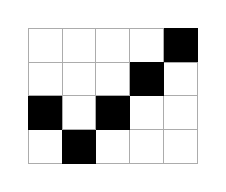
\begin{tikzpicture}[scale=.43]
\foreach \x in {0,...,5}{\draw[gray!65](\x,0)--(\x,4);}
\foreach \y in {0,...,4}{\draw[gray!65](0,\y)--(5,\y);}
\foreach \x/\y in {4/3,3/2,0/1,2/1,1/0}{\fill[black](\x,\y)rectangle +(1,1);}
\end{tikzpicture}\end{center}
This uses the initial-fill-as-output convention from the notes. The stream continues across row boundaries.

(c) \(x^4+x+1\) is irreducible and every nonzero fill has period 15, by the complete calculation in the LFSR-period topic. Quote the theorem's irreducibility and nonzero-fill hypotheses.

(d) Reusing a pad gives \(c\oplus c'=m\oplus m'\) for bits, or \(c-c'=m-m'\pmod{26}\) for letters. The secret pad cancels, exposing a relation between plaintexts.
\end{answer}
\begin{question}{Paper 3: RSA and the shared-prime attack}
Complete the RSA tasks and explain the company-wide weakness.
\end{question}
\begin{answer}{Paper 3}
(a) Choose distinct secret primes, compute \(N,\varphi(N)\), select coprime \(e\), find \(d\equiv e^{-1}\pmod{\varphi(N)}\); public \((N,e)\), private \(d\). Encrypt \(c=m^e\pmod N\), decrypt \(m=c^d\pmod N\). The RSA chapter gives correctness and the full computational method.

(b) Public \((85,11)\), private \(d=35\); message 4 encrypts to 64 and decrypts to 4. The repeated-squaring steps are shown in the RSA worked example.

(c) Signature \((m_0,\sigma)=(14,20)\), verified by \(20^3\equiv14\pmod{33}\).

(d) For three distinct primes, \(\gcd(p_ip_j,p_ip_k)=p_i\). Computing gcds between public moduli reveals their shared prime, hence both factors, totients and private exponents. When \(n\ge3\) and all pairwise products are published, every modulus shares a factor with another one. The degenerate \(n=2\) case has only one modulus and does not allow this pairwise-public-modulus attack; the company scenario presupposes enough primes/employees for overlap.
\end{answer}
\begin{question}{Paper 4: discrete logarithm and Dixon}
Complete both supplied algorithmic tasks.
\end{question}
\begin{answer}{Paper 4}
(a) BSGS gives \(\log_2 7=14\pmod{52}\), with baby index 6 and giant index 1 using \(m=8\). The complete lists and check appear in the BSGS topic.

(b) Discard seed 67, whose residue contains prime 13. For the retained seeds \((36,41,43,74)\), an exponent-parity matrix with factor-base rows \((2,3,5,7,11)\) is
\[E=\begin{bmatrix}0&1&1&1\\0&1&0&1\\0&0&1&0\\1&1&1&0\\1&1&0&0\end{bmatrix}.\]
Solving \(Ev=0\): row 3 gives \(v_3=0\); row 2 gives \(v_2=v_4\); row 5 gives \(v_1=v_2\). Thus a nonzero dependency is \((1,1,0,1)^\top\). It yields \(A=733,B_0=963\pmod{1219}\), and gcds 23 and 53. All full exponent factorizations and square-root construction appear in the Dixon topic.
\end{answer}
\begin{question}{Paper 5: simple noisy encryption and lattice attack}
Complete the five parts of the noisy-scheme question.
\end{question}
\begin{answer}{Paper 5}
(a) \(v=69\pmod{199}\). (b) Ciphertext \(e=18\). (c) \(b=54\), then \(r=3^{-1}54\equiv2\pmod8\).

(d) Use \(L=\Z(69,1)+\Z(199,0)\). It contains \((8,3)=3(69,1)-(199,0)\), a short vector compared with the given basis.

(e) Gauss steps are \((199,0)-3(69,1)=(-8,-3)\), followed by \((69,1)+8(-8,-3)=(5,-23)\). The final projection coefficient is \(29/73\), nearest integer 0. Thus \((-8,-3)\) is the shorter reduced basis vector, giving private key \((8,3)\) after a sign change. Its public congruence and decryption check establish the attack.
\end{answer}
\section{Non-examinable background: Enigma attacks and NTRU}
\begin{concept}{Enigma attacks: the role of conjugation and cribs}
The supplied exam guidance excludes the Attacking Enigma section. Its main lesson is that structure can defeat a huge nominal key space. A known plaintext fragment (a crib) can be aligned by rejecting positions where a letter would encrypt to itself. For guessed rotor settings, write the per-position maps as \(\sigma_i=P^{-1}Q_iP\), with unknown plugboard \(P\). Loops of plaintext/ciphertext relations imply fixed-point conditions on products of the \(Q_i\). Conjugate permutations have the same cycle type, so incompatible fixed-point/cycle data reject guesses without searching every plugboard.

In the simplified statistical model, a uniform permutation on 26 letters has expected one fixed point, and two independent ones have expected \(1/26\) common fixed points. Actual constraints and dependencies must be considered before treating those expectations as an exact success probability.
\end{concept}
\begin{concept}{NTRU: the notes' polynomial generalisation}
This section is also explicitly excluded from the exam. The notes replace integers with \(R=\Z[x]/(x^N-1)\), and use coefficient reductions \(R_p,R_q\). Multiplication in \(R\) wraps exponents using \(x^N=1\): cyclic convolution.

In the notation of these notes, short private polynomials \(s,t\) define public \(v=st^{-1}\in R_p\). Encrypt a small message polynomial \(r\) as \(e=qav+r\in R_p\). Multiplication by the private \(t\) gives \(te=qas+tr\), whose suitably small coefficient representatives can be lifted to the integer polynomial ring, then reduced modulo \(q\); multiplying by \(t^{-1}\in R_q\) recovers \(r\). Bounds and inverses are essential, just as in the simple noisy scheme.

This is a conceptual comparison using the lecture's notation, not a deployable cryptographic specification. In particular a polynomial with equally many +1 and -1 coefficients satisfies \(s(1)=0\); it cannot be a unit modulo \(x^N-1\). The notes' blanket demand that both \(s\) and \(t\) be invertible conflicts with that balanced choice. The displayed operations require inverses of \(t\); do not reproduce the inconsistent demand on \(s\) as an algebraic fact. No current security ranking is inferred from the lecture's informal historical remarks.
\end{concept}
\begin{tip}{Use your revision time according to the supplied guidance}
Do not memorise the full Enigma attack or NTRU protocol at the expense of BSGS, Dixon, RSA or Gauss reduction. Understand their place in the module, but the exam information explicitly excludes their sections.
\end{tip}
\begin{question}{Background check, not examinable}
Why can a polynomial with coefficient sum zero not be invertible modulo \(x^N-1\) over a field?
\end{question}
\begin{answer}{Background check}
Evaluation at \(x=1\) is a well-defined homomorphism on the quotient, because \(1^N-1=0\). If \(s(1)=0\) and \(su\equiv1\pmod{x^N-1}\), evaluation would give \(0\cdot u(1)=1\), a contradiction. Equivalently, \(s\) and \(x^N-1\) share factor \(x-1\).
\end{answer}
\section{Methods for unfamiliar questions and final revision checklist}
\begin{method}{Recognise the mathematical shape}
\begin{tabular}{p{.30\linewidth}p{.60\linewidth}}\toprule Trigger in the question&First action\\\midrule
A ciphertext and classical cipher type&Identify convention, recover a key, check the full plaintext\\
A table of shifted MutIoCs&Write \(k_i-k_j=\beta_{ij}\pmod{26}\)\\
A register recurrence&Write taps/polynomial, distinguish generation from period analysis\\
A public modulus appearing twice&Compute gcd with other public moduli\\
A large modular power&Repeated squaring; track the modulus\\
A congruence of two squares&Try both gcds with the modulus\\
Several smooth square residues&Find an exponent-parity dependency (Dixon)\\
A discrete log with moderate group order&BSGS, using \(q\) rather than the prime modulus\\
A collision with tracked exponents&Derive a linear congruence and handle nonunits\\
A smooth product of a shifted target&Take factor-base logs and subtract the shift\\
A small secret ratio modulo a prime&Construct \(\Z(v,1)+\Z(p,0)\), then Gauss-reduce\\\bottomrule
\end{tabular}
\end{method}
\begin{concept}{Security explanations: name a failure, exhibit its effect}
For each scheme, ask: What is public? What is private? What mathematical problem does the attacker face? What choice makes it easy? Can I turn that into a calculation?

Examples: reused OTP removes the pad; shared RSA primes yield a gcd; small-order DH gives few possible keys; repeated El-Gamal nonces expose a relation between plaintexts/signatures; short-vector reduction reveals the noisy scheme's trapdoor. Explain \emph{why} rather than writing only ``insecure''.
\end{concept}
\begin{tip}{A computational answer that is easy to mark}
State the algorithm, label the inputs and modulus, show a compact arithmetic table, identify the decisive collision/dependency/short vector, and verify the final result in the original equation. If a question names an algorithm, use it: a correct brute-force answer may not demonstrate the required skill. If stuck, state a valid setup and continue to other parts; the coursework explicitly values reasoned partial attempts.
\end{tip}
\begin{question}{Mixed unseen-style practice}
A company uses RSA moduli \(N_1=143,N_2=187\), and a colleague claims ``we have many key choices, so frequency analysis and shared-prime attacks cannot matter''. Identify two logically separate problems with this claim.
\end{question}
\begin{answer}{Mixed unseen-style practice}
First, key-space size alone is not a security proof: monoalphabetic substitution has \(26!\) keys yet preserves frequencies and patterns. Second, the published moduli share factor \(\gcd(143,187)=11\), so \(143=11\cdot13\) and \(187=11\cdot17\). Their totients are 120 and 160, allowing private exponents to be recovered from the public exponents. This is a concrete structural attack independent of the nominal number of available RSA keys.
\end{answer}

\section{Additional harder practice: transfer methods to unfamiliar cases}
\begin{question}{H.1: a known-plaintext stream attack}
A length-three LFSR has unknown taps \((b_0,b_1,b_2)\) and observed output \(100101\). Recover its taps. Explain why even a maximal-period LFSR is not a true one-time pad.
\end{question}
\begin{answer}{H.1}
Use \(a_{i+3}=b_0a_i+b_1a_{i+1}+b_2a_{i+2}\) in \(\F_2\). From \(a_0a_1a_2=100\) and \(a_3=1\), get \(b_0=1\). From \(a_1a_2a_3=001\), \(a_4=0\) gives \(b_2=0\). From \(a_2a_3a_4=010\), \(a_5=1\) gives \(b_1=1\). Thus the recurrence is \(a_{i+3}=a_i+a_{i+1}\), characteristic polynomial \(x^3+x+1\), with period 7 for nonzero fills.

Known plaintext and ciphertext reveal stream bits by XOR. Enough stream bits provide linear equations for taps and expose the fill. A maximal period describes repetition, not computational unpredictability. An OTP instead requires independent uniformly random key bits, with no short deterministic recurrence.
\end{answer}
\begin{question}{H.2: reducible LFSRs}
An LFSR has recurrence \(a_{i+4}=a_i+a_{i+2}\). Find the period for fill \(0101\) and explain why the irreducible-polynomial theorem is unavailable.
\end{question}
\begin{answer}{H.2}
Its polynomial is \(x^4+x^2+1=(x^2+x+1)^2\), so it is reducible. Starting \(0101\), the next bits are \(a_4=0+0=0\), \(a_5=1+1=0\), \(a_6=0+0=0\), \(a_7=1+0=1\). Continue: \(a_8=a_4+a_6=0\), \(a_9=a_5+a_7=1\). The first states are
\[0101,1010,0100,1000,0001,0010,0101.\]
The initial state first returns at time 6, so its period is 6. It need not divide 15 because irreducibility is absent. This explicit calculation also guards against trusting an incorrect visual-period claim without checking the recurrence.
\end{answer}
\begin{question}{H.3: an algebraic weakness of textbook RSA signatures}
Suppose raw RSA signatures satisfy \(\sigma_1^e\equiv m_1\), \(\sigma_2^e\equiv m_2\pmod N\). Give a signature on \(m_1m_2\pmod N\) without the private key. Explain why this is a limitation of the toy rule.
\end{question}
\begin{answer}{H.3}
Take \(\sigma=\sigma_1\sigma_2\pmod N\). Then
\[\sigma^e=(\sigma_1\sigma_2)^e\equiv\sigma_1^e\sigma_2^e\equiv m_1m_2\pmod N.\]
Thus signatures combine multiplicatively. More simply, choosing an arbitrary \(\sigma\) and setting \(m=\sigma^e\) creates a verifying pair, although it does not sign an arbitrary preselected meaningful document. These observations show why the course's raw arithmetic rule must not be mistaken for a complete secure document-signing construction. In exam answers distinguish forging \emph{some} valid pair from signing a specified target.
\end{answer}
\begin{question}{H.4: a complete index-calculus relation system}
In \((\Z/29\Z)^\times\) with generator 2 and factor base \(\{2,3,5\}\), use relations \(2^1\equiv2\), \(2^6\equiv6\), \(2^{13}\equiv14\), \(2^{23}\equiv10\). Which are usable? Recover all three base logs and then \(\log_2 15\).
\end{question}
\begin{answer}{H.4}
The order is 28. Discard \(14=2\cdot7\), which is not smooth over this base. Let \(u=\log_2 2,v=\log_2 3,w=\log_2 5\). The other relations give
\[u\equiv1,\quad u+v\equiv6,\quad u+w\equiv23\pmod{28}.\]
Thus \(u=1,v=5,w=22\pmod{28}\). Since \(15=3\cdot5\), \(\log_2 15\equiv5+22=27\pmod{28}\). Check \(2^{27}\equiv2^{-1}\equiv15\pmod{29}\). This target is smooth without a shift, so \(s=0\). The coefficient system happens to solve without dividing by a nonunit; do not assume every future system has that property.
\end{answer}
\begin{question}{H.5: exact key recovery versus a working replacement}
Gauss reduction gives a short lattice pair \((S,T)\) satisfying \(S\equiv Tv\pmod p\). Does this alone guarantee that it is Alice's original private key or that it decrypts every ciphertext?
\end{question}
\begin{answer}{H.5}
No. A lattice may contain several short candidates, and reduction can return a sign change or another vector. First check that \(S,T\) are coprime and in a range where modular multiplication does not wrap the quantity \(aS+Tr\) beyond \(p\), with the relevant signs and message bounds. Then use \(T^{-1}\pmod S\), which exists only under coprimality. If those conditions hold, the same algebra gives decryption with the replacement pair, even if it differs from the original key. A public congruence is necessary but is not the whole no-wraparound argument. In the supplied paper, the recovered positive pair is exactly \((8,3)\), so these checks are straightforward.
\end{answer}

\section{Source map and accuracy notes}
\begin{concept}{All four sources and how they were used}
\begin{enumerate}
\item \textbf{MATH6321 Notes(1).pdf}, Dr Dan Fretwell, 2026/27: Chapters 1--7 provide definitions, arithmetic conventions, scheme descriptions and algorithms. The appendix supplies English-frequency/MutIoC/ASCII reference material. This guide explains how to use letter-frequency tables and binary encodings rather than reprinting the large ASCII table.
\item \textbf{MATH6321 Exam Information.pdf}: governs the current two-hour structure, computational emphasis, supplied algorithms, and exclusions. These priorities override the older paper's timing.
\item \textbf{MATH6321 Coursework 1(1).pdf}: supplies the three cryptanalysis cases and the requirement to explain methods and verify recovered keys. Full worked cracking approaches appear in the coursework section.
\item \textbf{MATH320 Mathematical Cryptography Main Exam 24--25 (1).pdf}: the 2025 paper supplies worked Caesar/substitution/MutIoC, LFSR/picture/period, RSA, BSGS, Dixon and noisy-scheme examples. Its Useful Information sheets provide the supplied-algorithm conventions.
\end{enumerate}
The guide uses consistent row/column conventions and repairs algebraic slips rather than copying them: Gauss's angle is controlled by \(|u\cdot v|\le\|u\|^2/2\); a shortest vector has length \emph{at most} other nonzero vectors; and the NTRU background distinguishes the needed inverse of \(t\) from the contradictory balanced-\(s\) condition. The optional chi-square score is explained explicitly as an additional computational cryptanalysis aid. All model answers are independently derived.
\end{concept}
\end{document}
